% Requires running Bibtex

\documentclass[%
reprint,
amsmath,amssymb,
aps,
floatfix
]{revtex4-2}

\usepackage{graphicx}% Include figure files
\usepackage{dcolumn}% Align table columns on decimal point
\usepackage{bm}% bold math
\usepackage{hyperref}% add hypertext capabilities
\usepackage[font=scriptsize,labelfont=bf, justification=justified]{caption}% change fontsize in captions
\usepackage{float}
\usepackage{booktabs}% cool table style
\hypersetup{
	colorlinks=true,       % false: boxed links; true: colored links
	linkcolor=black,        % color of internal links
	citecolor=black,        % color of links to bibliography
	filecolor=black,     % color of file links
	urlcolor=black         
}

%\usepackage{bibspacing}
%\setlength{\bibitemsep}{.5\baselineskip plus .05\baselineskip minus .05\baselineskip}


\begin{document}
	
	\preprint{APS/123-QED}
	
	\title{PHYC30170 Physics with Astronomy and Space Science Lab 1;\\An Investigation of the Ramsauer-Townsend Effect}
	
	\author{Daragh Hollman}
	\email{daragh.hollman@ucdconnect.ie}
	
	\date{\today}
	
	\begin{abstract}
	The aims of this report were to investigate the Ramsauer-Townsend effect and determine the electron energy which yields a minimum probability of scattering. The contact potential and the emission electron energy were also determined to add to the accuracy of the measurement. The minimum probability of scattering was determined to be at electron energies of $(1.1 \pm 0.2) \,\text{eV}$. The contact potential was determined to be $(0.2 \pm 0.01) \,\text{V}$ and the emission electron energy was determined to be $(0.11 \pm 0.03) \,\text{V}$.
	\end{abstract}		
	
	\maketitle
	
	\section{Introduction}
	The Ramsauer-Townsend effect describes the phenomenon where electrons exhibit a minimum scattering cross section around electron energies of $1\,\text{eV}$ in noble gases \cite{wisconsin}. This interaction between particles cannot be described by a classical interpretation of particle collisions and requires a quantum mechanical description \cite{texas}. It is important to understand and experimentally test the Ramsauer-Townsend effect as to better understand how particle collisions work in quantum mechanics.
	
	\section{Theory}	
	Under classical mechanics, scattering particles are described by hard sphere scattering, where particles collide and interact as billiard balls might. Such a model is described in figure \ref{fig:hardSphereScattering} where the potential experienced by a light scattered particle is $U(r) = 0$ for $r > R$ and $U(r) = \infty$ for $r < R$ where $R$ is the radius of the sphere it scatters off \cite{santaBarbara}. It follows that, for a projectile particle moving towards the target but offset by a distance from the axis greater than $R$, the particle would not be deflected at all. We see there is some region with which the scattered particle cannot pass through, this area is known as the scattering cross section and when with respect to the total area it is analogous to the probability of scattering \cite{santaBarbara}.\\
	
	\begin{figure}
		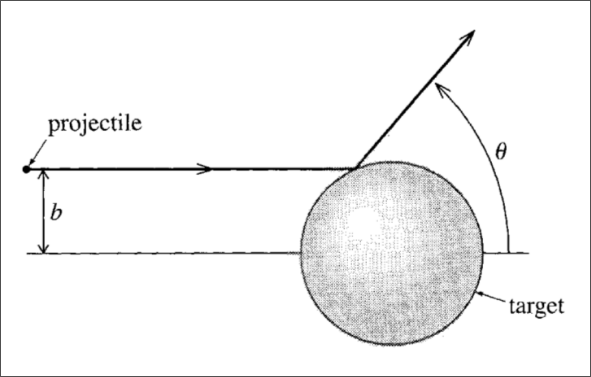
\includegraphics[width=0.85\columnwidth]{hardSphereScattering.png}
		\caption{\label{fig:hardSphereScattering}A simple hard sphere scattering model described by the potential $U(r) = 0$ for $r > R$ and $U(r) = \infty$ for $r < R$}
	\end{figure}
	
	When considered in this way, the scattering cross section of the noble gas atoms is independent of the incident electron energy. However, if the noble gas atoms are treated within quantum mechanics and present an attractive potential, akin to a square well, the solution of Schrödinger's equation yields that the scattering cross section will have a minimum for electron energies near $1 \,\text{eV}$ \cite{kukolich}\cite{sobhani}. The scattering of electrons by a square well can be predicted by a one-dimensional model or a three-dimensional model. These models represent the xenon atom as a square well with positive potential and are further described by Kukolich \cite{kukolich}.\\
	
	A thyratron, see figure \ref{fig:thyratron}, was used to demonstrate the Ramsauer-Townsend effect. The shield splits the cathode from the plate using two apertures. A beam of electrons starts at the cathode and moves towards the plate. After the first aperture, some electrons are scattered and don't arrive at the plate. In this region, the intensity of the electron beam is given as follows:
	\begin{equation}
		J = J_0 \exp{\left(-x \over \lambda \right)}
	\end{equation}where $x$ is the distance from the cathode and $\lambda$ is the mean free path \cite{kukolich}. The intensity at the plate is hence:
	\begin{equation}
		J_p = J_0 \exp{\left(-l \over \lambda \right)} = J_0 \left( 1 - P_s \right)
	\end{equation}where $l$ is the distance between the cathode and plate and $P_s$ is the probability of scattering \cite{kukolich}. As the shield current is proportional to the intensity of the electron beam at the first aperture, we can substitute the initial intensity, $J_0$, to obtain an expression for the plate current:
	\begin{equation}
		I_p = I_s f(V) (1-P_s)
		\label{eq:plateCurrent}
	\end{equation}where $I_p$ and $I_s$ are the plate and shield currents respectively, and $f(V)$ is a geometrical factor which depends on the ratio of angle intercepted by the plate to the angle intercepted by the shield and depends on a factor due to the space charge effects near the cathode \cite{kukolich}. This geometrical factor can be determined by cooling the xenon in the thyratron to reduce the pressure and eliminate scattering. $P_s$ goes to zero and hence:
	\begin{equation}
		f(V) \approx \frac{I_p^\star}{I_s^\star}
	\end{equation}where the $^\star$ notation indicates when cooled. Substituting the geometric factor back into equation \ref{eq:plateCurrent} we can solve for the probability of scattering.
	\begin{equation}
		P_s = 1 - \frac{I_p I_s^\star}{I_s I_p^\star}
		\label{eq:probability}
	\end{equation}\\
	
	\begin{figure}
		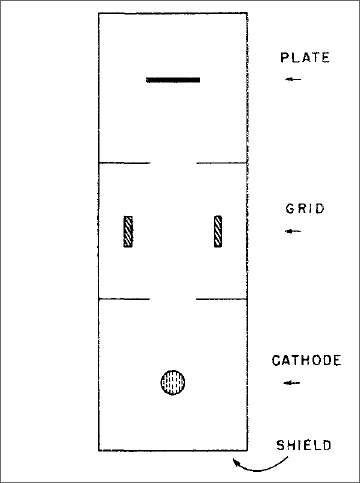
\includegraphics[width=0.65\columnwidth]{thyratron.png}
		\caption{\label{fig:thyratron}An example of a thyratron used in this experiment \cite{kukolich}.}
	\end{figure}
	
	A discrepancy in the data from the expected outcome is described by Kukolich and elaborated on by Woolsey \cite{kukolich} \cite{woolsey}. This discrepancy exists due to the contact potential and the emission energy of the thermionic electrons from the cathode. The contact potential arises from the shield and cathode being made from different metals which have different work functions. As the shield is made of nickel, it has a higher work function than the barium oxide cathode and hence as the two electrodes are in contact through the gas, there is a net flow of electrons to the shield without any potential \cite{woolsey}. To account for this, a negative potential at the shield is required to balance this flow. Hence the electrons leaving the cathode were affected by a total acceleration voltage of $(V + V_c)$ where $V_c$ is the contact potential between the electrodes. \\
	
	The emission energy of the thermionic electrons must also be accounted for. As the electrons leave the cathode they have a mean initial energy $e\bar{V} \,\text{eV}$ which also must be added to the acceleration voltage. Hence we have a total acceleration voltage of $(V + V_c + \bar{V})$ giving an electron energy of $(V - V_s + V_c + \bar{V})$. Woolsey describes the number of electrons with energy $\epsilon$ to be proportional to $\exp{\left( \frac{-\epsilon}{kT} \right)}$ \cite{woolsey}. Therefore for electrons with mean energy $\frac{3}{2}kT$ we have:
	\begin{equation}
		N(\epsilon) \propto \exp{\left( \frac{-3 V}{2 \bar{V}} \right)}
	\end{equation}which gives a current at the shield as follows:	
	\begin{equation}
		i = i_0 \exp{\left( \frac{-3 V_\text{accel}}{2 \bar{V}} \right)}
		\label{eq:slope}
	\end{equation}where $i_0$ is the current when the acceleration voltage, $V$, is zero.\\
	
	Therefore, to measure the probability of scattering as a function of electron momentum we must measure the potential across the plate resistor and across the shield resistor to find the plate and shield currents for a range of accelerating voltages and then repeat this when the thyratron is submerged in liquid nitrogen. To correct for the contact potential and the electron emission energy we must take measurements with the voltage source reversed.
	
	\section{Methodology}
	\subsection{Apparatus Setup}
	The apparatus was set up as shown in figure \ref{fig:circuit}. It contains a 2D21 thyratron pictured left which was set up such that the xenon tube could be submersed in liquid nitrogen for cooling. A funnel was used as a reservoir to ensure the tube remained submerged and at constant temperature (i.e. constant pressure) for the entire dataset. The thyratron consists of a cathode and a plate at opposite ends of the tube, across which the acceleration voltage is applied. This creates an electric field between the cathode and the plate. A filament at the cathode was heated by a constant $4 \,\text{V}$ to induce thermionic emission to free the electrons. \\
	
	\begin{figure}
		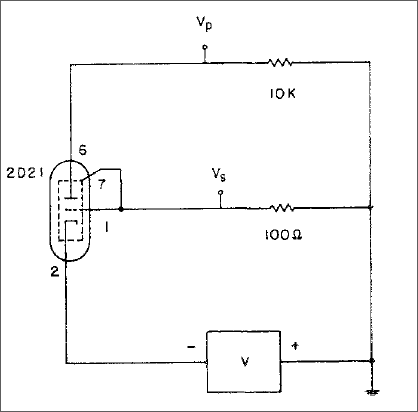
\includegraphics[width=0.85\columnwidth]{ramsauerCircuit.png}
		\caption{\label{fig:circuit}A circuit diagram of the experiment apparatus from Kukolich \cite{kukolich}.}
	\end{figure}
	
	\subsection{Procedure}
	The electronics were switched on in advance of taking the data to ensure the apparatus was not changing in temperature. Data was first collected for the thyratron at room temperature (xenon pressure $\approx 0.05 \,\text{Torr}$). The acceleration voltage was varied from $0 \,\text{V}$ to $15 \,\text{V}$ starting with steps of $0.1 \,\text{V}$ and changing to larger steps of $0.5 \,\text{V}$ after $2 \,\text{V}$. This ensured that the expected minimum around $1 \,\text{eV}$ in the scattering cross section would be well described. For each step, the acceleration voltage, plate voltage, and shield voltage were measured and recorded along with their respective uncertainties. The apparatus was then cooled using liquid nitrogen to reduce the pressure and the procedure was repeated.\\
	
	To account for the contact potential, $V_c$, and the emission energy of the thermionic electrons, $\bar{V}$, the voltage generator controlling the acceleration voltage was reversed such to drive the circuit with a negative potential to counteract the electron flow because of the contact potential. The shield current was recorded for voltages between $0 \,\text{V}$ and $-0.3 \,\text{V}$.
	
	\section{Results \& Analysis}
	The data recorded for the shield and plate voltage were converted to currents using Ohm's law. The plate currents, $I_p$ and $I_p^\star$, were plotted against the acceleration voltage as shown in figure \ref{fig:plateCurrentGraph}. The uncertainties on the voltages were propagated through Ohm's law to obtain uncertainties on the currents. The uncertainty on the voltage was limited by the accuracy of the multimeter. It is clear in this graph that the scattering is nullified when the thyratron is cooled by liquid nitrogen.\\
	
	\begin{figure}
		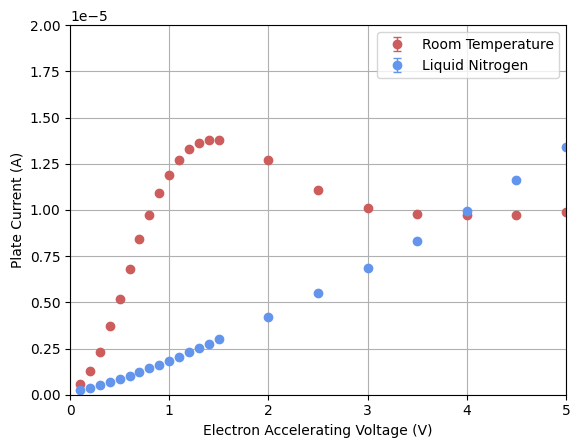
\includegraphics[width=\columnwidth]{plateCurrentGraph.png}
		\caption{\label{fig:plateCurrentGraph}Plate current against the acceleration voltage acting on the electron for both measurements, room temperature and liquid nitrogen cooled. Here the room temperature currents are multiplied by 10 to see them more easily. Note that error bars are present but are too small to see.}
	\end{figure}
	
	Using equation \ref{eq:probability}, the probability of scattering was determined as a function of electron momentum. This is plotted in figure \ref{fig:probabilityOfScattering}. Once again, the uncertainties here are propagated through the relevant equations to yield the uncertainties plotted on the data. Two distinct minima can be seen in the data. The first of which is just below $1 \,\text{eV}$ due to the Ramsauer-Townsed effect, and second at the point of ionisation. The minimum probability of scattering due to the Ramsauer-Townsend effect was determined by fitting an inverted Gaussian function in the range of $0.3 \,\text{V}$ to $1.3 \,\text{V}$. This was done through least squares fitting. The minimum point occurred at $(0.794 \pm 0.002) \,\text{V}$ with the uncertainty being determined by the square root of the diagonal elements of the covariance matrix of this Gaussian fit.\\ 
	
	\begin{figure}
		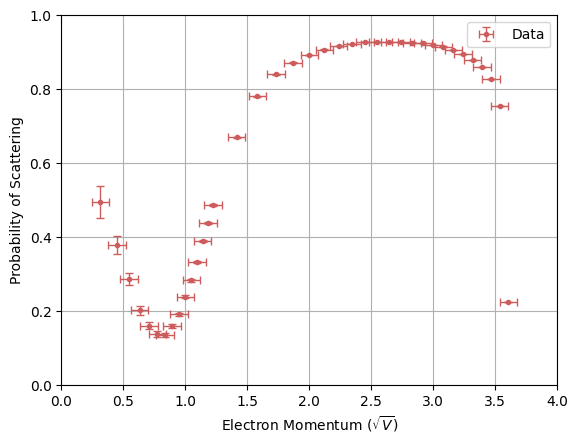
\includegraphics[width=\columnwidth]{probabilityOfScattering.png}
		\caption{\label{fig:probabilityOfScattering}The probability of scattering against the electron momentum. Note that this is unadjusted for contact potential and electron initial energy.}
	\end{figure}
	
	To calculate the contact potential and the emission energy of the thermionic electrons, the data from the reverse acceleration voltage measurement was plotted in figure \ref{fig:kneeGraph}. $\log{I_s^\star}$ was plotted against the reverse acceleration voltage. We see a straight line which gets steeper after the potential balances that of the contact potential. This turnover point is a measurement of the contact potential. Two exponential lines were fitted using least squares fitting to each portion of the data to determine the intersection point. The contact potential was determined to be $(0.2 \pm 0.01) \,\text{V}$, the uncertainty on which was determined by the method of extremes. $\bar{V}$ can also be determined from this graph. Using equation \ref{eq:slope}, $\bar{V}$ was determined to be $(0.11 \pm 0.03) \,\text{V}$. The calculation of both of these values from the graphs is included in full in appendix A. From these values, a final determination of the electron energy yielding a minimum probability of scattering is at $(1.05 \pm 0.2) \,\sqrt{\text{V}}$.
	
	\begin{figure}
		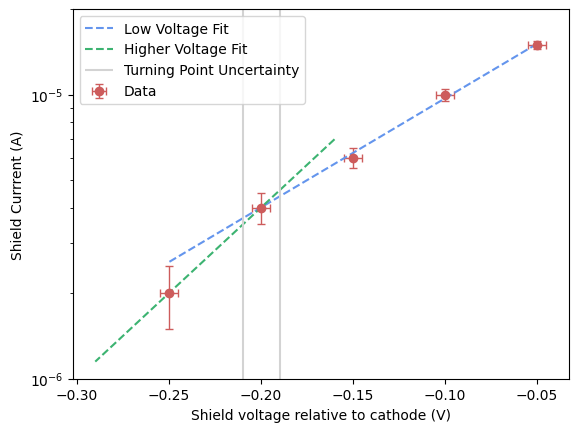
\includegraphics[width=\columnwidth]{kneeGraph.png}
		\caption{\label{fig:kneeGraph}The shield current against the accelerating voltage in reverse. Note that due the lack of a higher precision ammeter, data below $-0.25 \,\text{V}$ could not be measured.}
	\end{figure}
	
	\section{Conclusion}
	The aims of this report were to investigate the Ramsauer-Townsend effect and determine the electron energy which yields a minimum probability of scattering. The contact potential and the emission electron energy were also determined to add to the accuracy of the measurement. The minimum probability of scattering was determined to be at electron energies of $(1.1 \pm 0.2) \,\sqrt{\text{V}}$. This agrees well with the analytical findings of Vahedi \cite{vahedi} and Kukolich \citep{kukolich} that the electron energy should be around $1 \,\text{eV}$. The contact potential was determined to be $(0.2 \pm 0.01) \,\text{V}$ and the emission electron energy was determined to be $(0.11 \pm 0.03) \,\text{V}$.
		
		
	\clearpage
	\bibliography{ramsauer.bib}% Produces the bibliography via BibTeX.
	
	\clearpage
	\onecolumngrid
	\appendix
	
	\section{Calculation of $V_c$ and $\bar{V}$}
	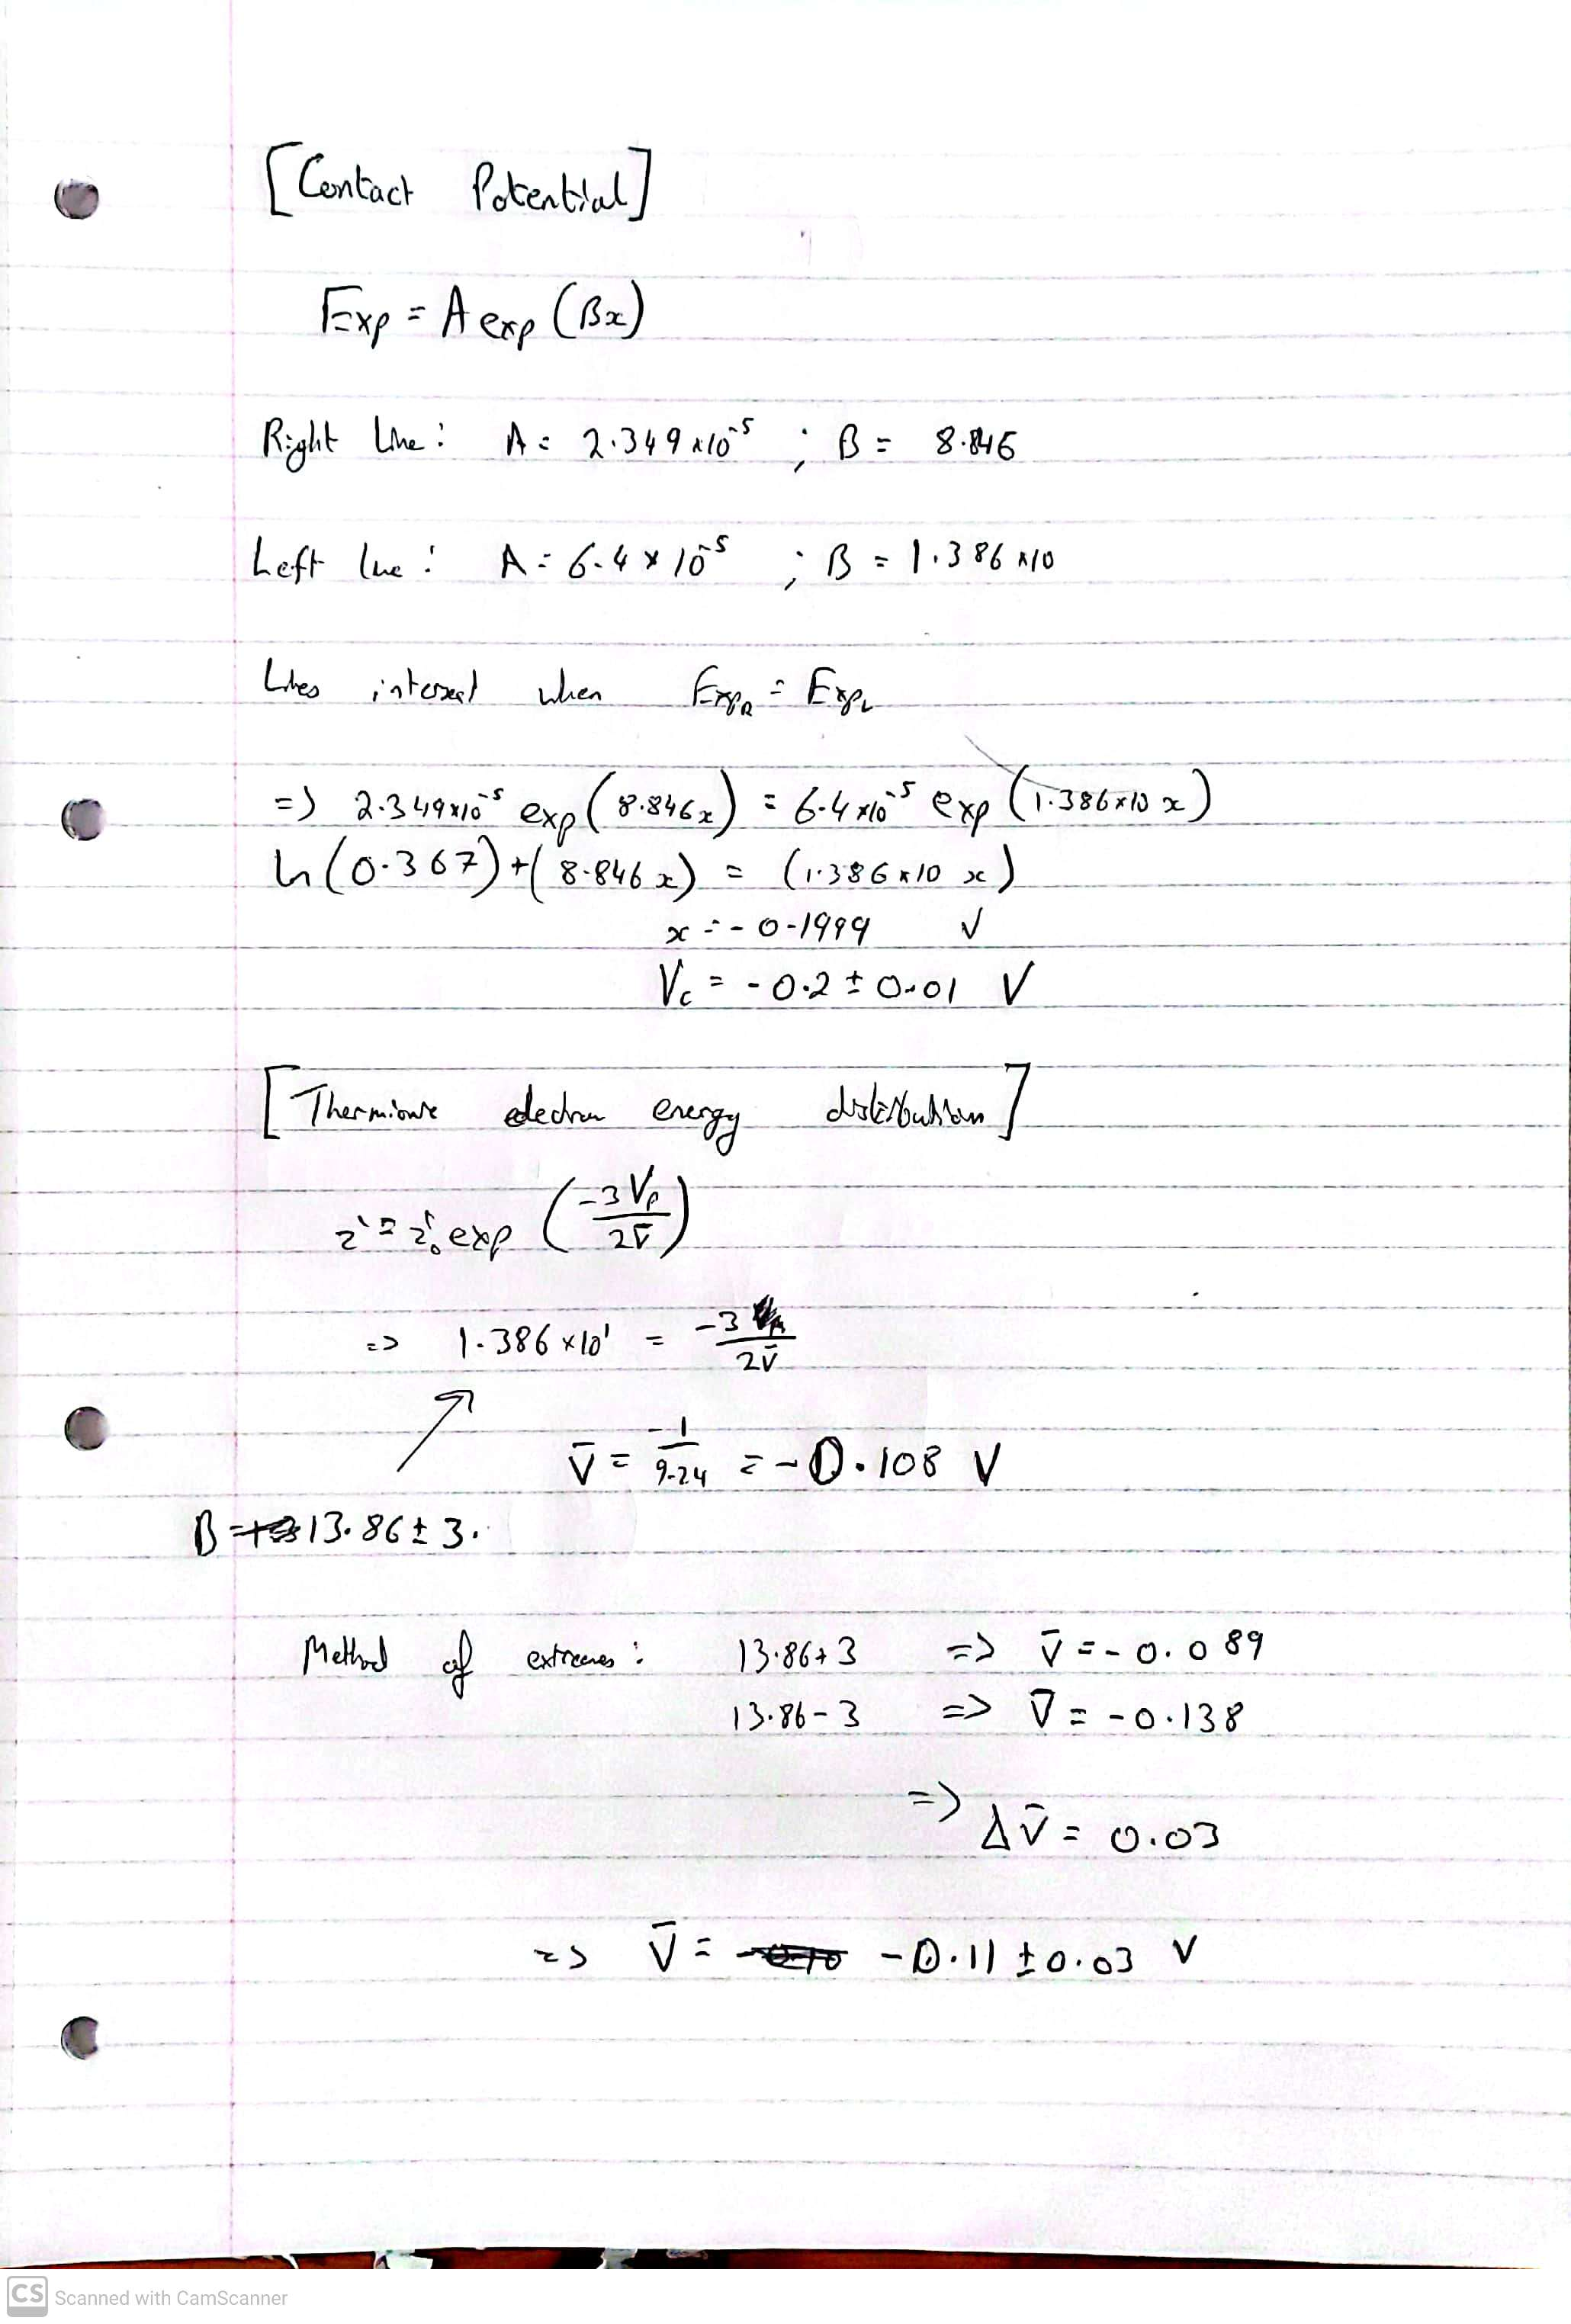
\includegraphics[width=0.9\columnwidth]{discrepancies.jpg}

	
	
\end{document}

